\documentclass[12pt,a4paper,titlepage,brazil]{article}
\usepackage{tabularx}
\usepackage{graphicx}
\usepackage[brazilian]{babel} 
\usepackage[T1]{fontenc}
\usepackage[utf8]{inputenc}
\usepackage[a4paper]{geometry}
\geometry{top=2.5cm, bottom=2.5cm, left=3.0cm, right=2.0cm}
\usepackage{setspace}
\usepackage{titleps}
\usepackage{amsmath}
\usepackage{libertine}
\usepackage{hyperref}
\usepackage{tikz}
\usepackage[thicklines]{cancel}
\usepackage{tcolorbox}%para fazer caixas no texto - Gera caixas em escalas de cinza
%\newtcolorbox{mybox}{colback=red!5!white,colframe=red!75!black}%gera caixas com as cores definidas
\newtcolorbox{mybox1}[1]{colback=red!5!white,colframe=red!75!black,fonttitle=\bfseries,title=#1}%um tipo customizado de caixa com titulo e cores
\newtcolorbox{mybox2}[1]{colback=green!5!white,colframe=green!75!black,fonttitle=\bfseries,title=#1}%um tipo customizado de caixa com titulo e cores

%Cabeçalho e o rodapé
\newpagestyle{ruled}
{\sethead{}{Minicurso: Introdução à relatividade}{}\headrule
  \setfoot{}{Natalí Soler Matubaro de Santi --- natalidesanti@gmail.com}{}\footrule}
\pagestyle{ruled}

%-----------------------------------------------------------------------

\begin{document}

\begin{center}
 \LARGE{\bf Introdução à relatividade}
\end{center}

%------------------------------------------------------------------------

Estas notas de aula tem o intuito de proporcionar um panorama geral de Relatividade Especial (RE) e Relatividade Geral (RG). Por este motivo elas não são completas (com todas as deduções e tópicos usualmente abordados em cursos de RE ou mesmo RG) e não possuem um formalismo matemático tão rebuscado. Resolvi focar nos conceitos físicos motivacionais e primordiais, ao meu ver, de ambas teorias para aquelas pessoas que desejam uma {\bf Introdução à Relatividade}. Portanto, não pretendem ser um curso completo de Relatividade.

Minha recomendação para um estudo mais aprofundado em Relatividade consiste na leitura parcial e/ou completa dos seguintes livros, apresentados aqui em nível de dificuldade do mais básico para o mais avançado:

\begin{itemize}
 \item {\em Introduction to elementary particles} de D. Griffiths \cite{particulas} - embora seja um livro de Física de Partículas apresenta uma linguagem divertida e compreensível para uma primeira interação com relatividade especial, já apresentando a notação covariante. Possui uma gama de exemplos comentados;
 \item {\em A Short Course in General Relativity} de J. Foster e J. D. Nightingale \cite{nightingale2006} - fornece uma excelente revisão em RE em um de seus apêndices, mesmo para iniciantes em RE. No geral consiste em um excelente curso de RG. Possui uma série de interessantes exercícios e apresenta a resolução dos mesmos em outro de seus apêndices;
 \item {\em Spacetime and Geometry: An introduction to general relativity} de S. M. Carroll \cite{carroll2004} - apresenta RE e RG com uma linguagem divertida e muito acessível. Vai além, em questão de formalismo matemático, tópicos e conceitos físicos, se comparado às referências anteriores;
 \item {\em Gravity: An introduction to Einstein’s general relativity} de J. B. Hartle \cite{hartle2003}- é comparável a referência anterior, apresentando um ponto a mais: é uma excelente pedida para quem quer se aventurar usando RG para resolução de problemas numéricos usando o software \texttt{Mathematica}.
 \item {\em General Relativity} de R. M. Wald \cite{wald2010} - esta referência é matematicamente muito bem formulada e avançada. Recomendo para quem deseja lidar com formalismo matemático avançado.
\end{itemize}  

% --------------------------------------------------------------------

\section{Introdução}

Isaac Newton acreditava que o espaço e o tempo eram entidades completamente separadas: o tempo fluiria igualmente para todos os observadores e as distâncias espaciais seriam idênticas independentemente do que esses observadores fizessem. A {\bf Dinâmica Newtoniana}, consolidada na publicação de seu livro {\em Philosophiae Naturalis Principia Mathematica} (1687), funciona muito bem para fenômenos cotidianos, como para descrever movimentos simples (trajetória de carros, corredores, bolas de futebol) \cite{nightingale2006}.

Entretanto, no início do século XX a {\bf Teoria da Relatividade} surgiu, revolucionando a Física existente até o momento \cite{pires2011}. Noções de que o espaço e o tempo seriam partes de uma entidade única e fundamental, o espaço-tempo, nortearam o desenvolvimento da RE \cite{einstein1905, martins2005}. Essa teoria impunha que as leis da Física seriam as mesmas em todos os referenciais inerciais e que a velocidade da luz seria um limite natural independente do referencial em questão. Dessa forma, ela confrontava as tão bem estabelecidas {\bf Leis de Newton}, porque, segundo as mesmas, a interação gravitacional agiria instantaneamente. Assim, a ideia de unir a RE à gravitação foi uma das bases para o desenvolvimento da RG.

Em 1915 Albert Einstein propôs uma série de equações que consolidaram a RG \cite{einstein1915}. A RG pode ser descrita como uma teoria da gravitação que proporciona uma nova conotação para a gravidade: ela não seria mais considerada como uma força entre dois corpos, como na teoria Newtoniana, mas sim uma manifestação da curvatura do espaço-tempo. Além disso, essa teoria mantinha as noções de causalidade e localidade da RE. Diversos testes e experimentos foram e ainda são feitos com essa teoria, a saber: o avanço no periélio de Mercúrio, a deflexão e o desvio espectral da luz e, mais recentemente, as ondas gravitacionais, obtendo extrema precisão experimental. Em 1916, a primeira solução para as equações de Einstein foi criada por Karl Schwarzschild \cite{schwarzschild1916} e após muita relutância, ela foi o ponto de partida para a teoria dos buracos negros.

%------------------------------------------------------------------------

\section{Relatividade especial}

A RE ou {\bf Relatividade Restrita} é o estudo das propriedades geométricas do espaço-tempo na ausência de {\em campos gravitacionais} e de seus efeitos nos fenômenos físicos que nele se desenvolvem \cite{particulas, nightingale2006, carroll2004}.\\

\begin{tcolorbox}
 {\bf Observadores/referenciais inerciais} são sistemas de coordenadas baseados em três eixos mutualmente ortogonais, de coordenadas, por exemplo, $x$, $y$ e $z$ no espaço, e um sistema de relógios sincronizados no repouso para esse sistema, que fornece um tempo $t$. Esse sistema é construído de modo que o movimento de uma partícula formulado para esse sistema assegura a {\em primeira lei de Newton}: objetos continuam a se mover em linhas retas e com velocidades constantes a menos que uma força atue sobre eles. 
\end{tcolorbox}

Os postulados fundamentais da RE podem ser descritos como:
\begin{enumerate}
 \item A velocidade da luz $c$ é a mesma em todos os referenciais inerciais;
 \item As leis da natureza são as mesmas em todos os referenciais inerciais.
\end{enumerate}  

Dado o primeiro postulado da RE podemos traduzi-lo pensando em dois referenciais inerciais $S$ e $S'$ de forma que
\begin{equation}
 c = \frac{d r}{ d t} = \frac{d r'}{d t'} \label{eq:c1}
\end{equation}  
onde $dr^2 = dx^2 + dy^2 + dz^2$ e $dr'^2 = dx'^2 + dy'^2 + dz'^2$. Assim, podemos reescrever (\ref{eq:c1}) como
\begin{equation}
 c^2 d t^2 - d x^2 - d y^2 - d z^2 = c^2 (d t')^2 - (d x')^2 - (d y')^2 - (d z')^2 = 0 .
\end{equation}
Isso nos leva a assumir um {\bf intervalo invariante} $d s^2$ entre esses dois eventos, de modo que
\begin{equation}
 d s^2 = c^2 d t^2 - d x^2 - d y^2 - d z^2 = c^2 (d t')^2 - (d x')^2 - (d y')^2 - (d z')^2 , \label{eq:ds2}
\end{equation}
que vale $d s^2 = 0$, quando pensamos na trajetória de um fóton, partícula de luz. Essa quantidade $d s^2$ é, de fato, conhecida como {\bf intervalo invariante} em relatividade e possui o mesmo valor em qualquer referencial inercial. Veja que, por outra convenção estabelece-se o {\bf intervalo invariante} com sinais trocados, ou seja, atribui-se o sinal negativo à coordenada temporal e o sinal positivo às coordenadas espaciais. Faremos uso dessa outra convenção na dedução da solução de Schwarzschild.

%------------------------------------------------------------------------

\subsection{Transformações de Lorentz}

Dados dois referenciais inerciais $S$ e $S'$, temos $S'$ se movendo a uma velocidade uniforme ${\bf v}$ (de magnitude $v$) com respeito a $S$ e, então, $S$ se movendo com velocidade $- {\bf v}$ com respeito a $S'$. Tomando o movimento apenas na direção $x$ (ver Figura \ref{fig:lorentz}), vamos considerar os relógios coincidindo seu instante zero $t = t' = 0$ quando $x = x' = 0$. Supondo que algum evento ocorra na posição $(x, y, z)$, no tempo $t$ em $S$, quais serão as coordenadas espaço-temporais de ocorrência desse mesmo evento para o referencial $S'$?

\begin{figure}[h!]
 \centering
 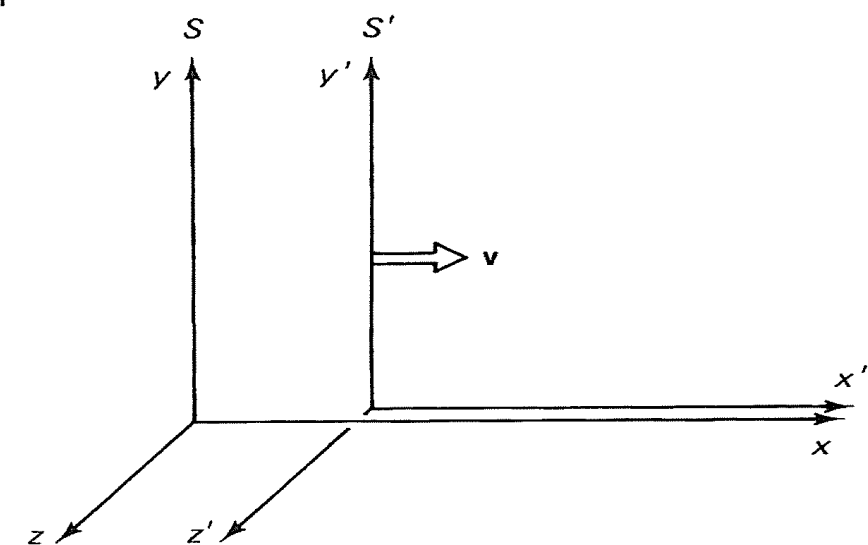
\includegraphics[scale=0.3]{figuras/lorentz.png}
 \caption{Sistemas inerciais das transformações de Lorentz.\label{fig:lorentz}}
\end{figure}

A resposta para essa pergunta é dada pelas {\bf Transformações de Lorentz}:
\begin{align}
 x' & = \gamma \left( x - v t \right) \label{eq:L1}\\
 t' & = \gamma \left( t - \frac{v}{c^2} x \right) \label{eq:L2}\\
 y' & = y \label{eq:L3}\\
 z' & = z \label{eq:L4}
\end{align}
onde
\begin{equation}
 \gamma = \frac{1}{\sqrt{1 - \frac{v^2}{c^2}}} .
\end{equation}
O fator $\gamma$ é tal que $\gamma > 1$ porque sempre $v < c$. No caso de $v \ll c$, diz-se que temos o limite não relativístico, no qual $\gamma = 1$.

A transformação inversa, de $S'$ para $S$ é dada por
\begin{align}
 x & = \gamma \left( x' + v t' \right) \label{eq:IL1}\\
 t & = \gamma \left( t' + \frac{v}{c^2} x' \right) \label{eq:IL2}\\
 y & = y' \label{eq:IL3}\\
 z & = z' \label{eq:IL4}
\end{align}

\begin{tcolorbox}
  {\bf Exercício 1:} Mostre que a transformação inversa das transformações de Lorentz é dada pelas equações \ref{eq:IL1}, \ref{eq:IL2}, \ref{eq:IL3} e \ref{eq:IL4}.

  {\bf Dica:} Resolva o sistema de equações gerado pelas próprias equações da transformação de Lorentz (\ref{eq:L1}, \ref{eq:L2}, \ref{eq:L3} e \ref{eq:L4}) para $x$, $y$, $z$ e $t$. 
\end{tcolorbox}

%------------------------------------------------------------------------

\subsection{Dilatação temporal}

Vamos considerar o referencial inercial $S'$, onde dois eventos $(x_1', t_1')$ e $(x_2', t_2')$ acontecem na mesma posição, i.e.,
\begin{equation}
 \Delta x' = x_2' - x_1' = 0 .
\end{equation}
O tempo entre esses dois eventos, medidos por $S'$ é
\begin{equation}
 \Delta t' = t_2' - t_1' .
\end{equation}
Para o referencial $S$ temos
\begin{align}
 \Delta x & = x_2 - x_1 \neq 0 ,\\
 \Delta t & = t_2 - t_1 .
\end{align}
Mas como podemos associar as medidas de tempo entre os referenciais?

A resposta pode ser dada pelas transformações de Lorentz:
\begin{align}
 x_1' & = \gamma \left( x_1 - v t_1 \right) ,\\
 x_2' & = \gamma \left( x_2 - v t_2 \right) ,\\
 t_1' & = \gamma \left( t_1 - \frac{v}{c^2} x_1 \right) ,\\
 t_2' & = \gamma \left( t_2 - \frac{v}{c^2} x_2 \right) ,
\end{align}
implicando que
\begin{align}
 \Delta x' & = \gamma \left( \Delta x - v \Delta t \right) = x_2' - x_1' = 0 \hspace{0.2cm}\Rightarrow\hspace{0.2cm} \Delta x = v \Delta t \\
 \Delta t' & = \gamma \left( \Delta t - \frac{v}{c^2} \Delta x \right) = \gamma \left( \Delta t - \frac{v}{c^2} v \Delta t \right) = \gamma \left( 1 - \frac{v^2}{c^2} \right) \Delta t .
\end{align}  
Portanto,
\begin{equation}
 \Delta t = \gamma \Delta t' ,
\end{equation}
ou seja, como $v < c$ e, então $\gamma > 1$, na percepção do referencial $S$ os dois eventos demoram mais para passar do que para o referencial $S'$ $\Rightarrow$ temos uma {\bf dilatação temporal}!

%------------------------------------------------------------------------

\subsection{Contração espacial}

Vamos considerar um objeto, de comprimento $l'$, em repouso no referencial inercial $S'$, ou seja, ele estará se movendo com velocidade $v$ com relação ao referencial $S$. Queremos medir seu comprimento com relação ao referencial inercial $S$.

No referencial $S'$ uma das extremidades do objeto possui posição $x_1'$ e a outra $x_2'$, então seu comprimento é dado por $\Delta x' = x_2' - x_1'$. Como no referencial $S'$ o objeto está em repouso, o comprimento deste objeto neste referencial inercial é equivalente a seu {\em comprimento próprio}, i.e., $l'$.

Para o referencial $S$ o objeto está em movimento, então seu comprimento, medindo suas extremidades em $x_1$ e $x_2$ é dado por
\begin{equation}
 \Delta x = x_2 - x_1.
\end{equation}
É claro, que como em qualquer medida $x_1$ e $x_2$ são aferidos {\em ao mesmo tempo}, ou seja,
\begin{equation}
 \Delta t = t_2 - t_1 = 0. \label{eq:dt=0}
\end{equation}

Uma medida simultânea no referencial inercial $S$ não é simultânea no referencial inercial $S'$ porque um está em movimento com relação ao outro. Mas como podemos associar as medidas de espaço entre os dois referenciais?

Novamente a resposta é dada fazendo uso das {\em Transformações de Lorentz}:
\begin{align}
 x_1' & = \gamma \left(x_1 - v t_1\right)\\
 x_2' & = \gamma \left(x_2 - v t_2\right) .
\end{align}
Como $t_1 = t_2$ \ref{eq:dt=0}, escrevemos
\begin{equation}
 \Delta x' = \gamma \Delta x \hspace{0.1cm}\Rightarrow\hspace{0.1cm} \Delta x = \frac{\Delta x}{\gamma} .
\end{equation}
Portanto, o comprimento do objeto em repouso no referencial inercial $S'$, mas em movimento para o referencial inercial $S$, é menor para o referencial inercial $S$ $\Rightarrow$ temos uma {\bf contração espacial}!

%------------------------------------------------------------------------

\subsection{Dinâmica relativística: conservação de energia e momentum}

%%%
\subsubsection{Energia e momentum}

Já falamos do {\em comprimento próprio}, o comprimento de um objeto em seu referencial de repouso. Em relatividade, damos o nome de {\bf tempo próprio} $\tau$ para o tempo de um observador em repouso com relação a um referencial inercial. Podemos relacionar o tempo próprio $\tau$ com o tempo de outro referencial $t$, infinitesimalmente, como
\begin{equation}
 d \tau = \frac{d t}{\gamma} .
\end{equation}
Normalmente, para velocidades muito menores que a da luz ($v \ll c$), $\gamma = 1$, então não há diferenças entre os tempos medidos. É interessante olharmos para o tempo próprio $\tau$ porque ele é invariante, i.e., todos os observadores que tiverem acesso ao tempo próprio $\tau$ de um outro observador ou corpo farão a mesma medida de tempo, mesmo se seus relógios diferirem uns dos outros.

Quando falamos da velocidade $v$ de um corpo, com relação ao laboratório, estamos falando do quanto o mesmo andou (variação de espaço medido com relação ao laboratório) com relação ao tempo (também com relação ao laboratório), ou seja,
\begin{equation}
 {\bf v} = \frac{d {\bf x}}{d t} .
\end{equation}  
Mas também podemos expressar a {\bf velocidade própria} desse corpo como
\begin{equation}
 {\bf u} = \frac{d {\bf x}}{d \tau} = \gamma {\bf v} .
\end{equation}  
Em certo sentido essa é uma quantidade híbrida: mistura o quanto o corpo andou no referencial do laboratório, com relação ao tempo próprio: mas lembre-se que, no referencial em que o corpo está em repouso, ele nunca se move. Assim, essa definição necessariamente deve ser ``híbrida''.

A definição de {\bf momentum} ${\bf p}$ implica que queremos que o mesmo se conserve e que obedeça o primeiro princípio da RE, portanto, definimos
\begin{equation}
 {\bf p} \equiv m {\bf u} = \gamma m {\bf v} = \frac{m {\bf v}}{\sqrt{1 - \frac{v^2}{c^2}}}.
\end{equation}
É importante notar que, para $v \ll c$, $\gamma = 1$ e, portanto, recuperamos a definição clássica de momentum: ${\bf p} = m {\bf v}$.

A definição de {\bf energia} fica então dada por
\begin{equation}
 E \equiv \gamma m c^2 = \frac{m c^2}{\sqrt{1 - \frac{v^2}{c^2}}}.
\end{equation}
Essa expressão não recai exatamente na expressão clássica para energia quando $v \ll c$. Porém, podemos expandir essa expressão em Taylor, na variável $\frac{v}{c}$ ao redor de zero, obtendo:
\begin{equation}
 E = m c^2 \left[1 + \frac{1}{2} \frac{v^2}{c^2} + O\left(\frac{v^4}{c^4}\right)\right] \simeq m c^2 + \frac{1}{2} m v^2 .
\end{equation}
O primeiro termo dessa expansão é chamado de {\bf energia de repouso}
\begin{equation}
  R \equiv m c^2 
\end{equation}  
e representa a energia de um objeto para quando $v = 0$. Já o segundo termo em diante representa a {\bf energia cinética}
\begin{equation}
 T \equiv m c^2 (\gamma - 1) \simeq \frac{1}{2} m v^2 + O\left(\frac{v^4}{c^4}\right)
\end{equation}
desse objeto e, seu primeiro termo, é exatamente a expressão clássica para a energia cinética de um corpo de massa $m$ e velocidade $v$.
Então, ficamos com
\begin{equation}
 E = \frac{m c^2}{\sqrt{1 - \frac{v^2}{c^2}}} \hspace{1cm}\textnormal{e}\hspace{1cm} {\bf p} = \frac{m {\bf v}}{\sqrt{1 - \frac{v^2}{c^2}}}. \label{eq:EPm}
\end{equation}  
Portanto, podemos escrever a seguinte expressão para a conservação de energia e momentum de um objeto relativístico de massa $m$ e momentum ${\bf p}$ como
\begin{equation}
 E^2 = m^2 c^4 + {\bf p}^2 c^2 . \label{eq:consE-P}
\end{equation}

\begin{tcolorbox}
 {\bf Exercício 2:} Mostre que a expressão (\ref{eq:consE-P}) é válida substituindo as expressões de energia e momentum (\ref{eq:EPm}).
\end{tcolorbox}

Mas o que acontece para um objeto sem massa ($m = 0$)? Ele não possui energia e nem momentum? A equação (\ref{eq:consE-P}) implica que, quando $m = 0$, temos
\begin{equation}
 v = c \hspace{1cm}\textnormal{e}\hspace{1cm} E = |{\bf p}| c .
\end{equation}  
Mas como os fótons se diferenciam uns dos outros? A relatividade apenas diz que é devido a momentum $|{\bf p}_1| \neq |{\bf p}_2|$ diferentes. Entretanto, quanticamente, podemos diferenciar os fótons a partir de sua frequência $\nu$ de forma que
\begin{equation}
 E = h \nu .
\end{equation}  
Portanto, maiores frequências (azul) implicam em maiores energias, enquanto menores frequências (vermelho), implicam em menores energias.

%%%
\subsubsection{Conservação de energia e momentum - Colisões}

Em RE quando falamos de colisões implicamos nas conservações básicas de energia e momentum. A principal diferença, comparada a colisões clássicas, é que em RE a massa não é conservada, ou seja, ela pode ser transformada em energia cinética, ou vice versa, dado que agora massa equivale a energia, a energia de repouso de um objeto.\\

\textbf{Exemplo}

Duas partículas, cada uma de massa $m$ e velocidade igual a $v = \frac{3}{5} c$, colidem frontalmente e permanecem juntas em repouso com uma massa final $M$. Qual é a massa final $M$?

\begin{figure}[h!]
 \centering 
 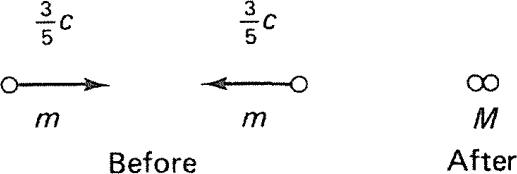
\includegraphics[scale=0.5]{figuras/ex1.png}
 \caption{Colisão de duas partículas de massa $m$ e velocidades $\frac{3}{5} c$, formando uma partícula em repouso de massa $M$.}
\end{figure}

Caso $v \ll c$ a resposta para essa pergunta seria óbvia: $M = 2 m$. Porém, aqui estamos lidando com uma situação relativística porque $v = \frac{3}{5} c$.

Nesse caso a conservação de momentum é trivial e não fornece nenhuma informação sobre a massa da partícula $M$:
\begin{equation}
 {\bf p}_M = {\bf p}_m^1 + {\bf p}_m^2 = 0 \Rightarrow {\bf p}_m^1 = - {\bf p}_m^2 .
\end{equation}
Já a conservação de energia implica que
\begin{equation}
 E_M = E_m^1 + E_m^2 = 2 E_m^1 = 2 E_m^2 = 2 E_m
\end{equation}
ou seja,
\begin{equation}
 M c^2 = 2 E_m = \frac{2 m c^2}{\sqrt{1 - \left(\frac{3}{5}\right)^2}} = \frac{5}{2} m c^2 ,
\end{equation}
portanto
\begin{equation}
 M = \frac{5}{2} m .
\end{equation}  
Veja que $M$ ficou maior que a $2 m$, porque a energia cinética se transformou em energia de repouso, ou seja, em massa.

%------------------------------------------------------------------------

\subsection{Notação covariante}
\label{subsec:not_cov}

Até agora não vimos nada sob um ponto de vista matematicamente mais rebuscado, o que, em RE, é chamado de {\bf notação covariante}. Essa notação existe com o intuito de, além de fornecer uma sofisticação matemática, estabelecer os postulados da relatividade, simplificar as contas de problemas mais complicados, como por exemplo, para problemas de colisões e já introduzir a notação utilizada em RG.

Vamos introduzir o 4-vetor posição $x^{\mu}$, com $\mu = 0, 1, 2, 3$, como sendo
\begin{equation}
 x^0 = c t, x^1 = x, x^2 = y, x^3 = z . \label{eq:contrav}
\end{equation}
Usualmente representa-se com letras latinas ($i$, $j$, $k$, $l$, $\dots$) as coordenadas espaciais, valendo $1$, $2$ ou $3$, e com letras gregas as ($\mu$, $\nu$, $\alpha$, $\beta$, $\dots$) coordenadas temporais e espaciais, valendo $1$, $2$, $3$ ou $4$. Podemos traduzir o {\bf intervalo invariante} $d s^2$, visto na equação (\ref{eq:ds2}), com esta notação como
\begin{equation}
  d s^2 = g_{\mu \nu} d x^{\mu} d x^{\nu} = g_{\mu \nu} d x'^{\mu} d x'^{\nu} ,
\end{equation}  
onde
\begin{equation}
  [g_{\mu \nu}] = \left[\begin{array}{cccc}
                          1 & 0 & 0 & 0\\
                          0 & - 1 & 0 & 0 \\
                          0 & 0 & - 1 & 0 \\
                          0 & 0 & 0 & - 1
                                      \end{array}\right] . \label{eq:gmunu-P}
\end{equation}
A quantidade $g_{\mu \nu}$ é conhecida como {\bf tensor métrico}\footnote{O tensor métrico possui uma série de propriedades muito importantes e úteis em RE e em RG, sendo a quantidade primordial desta última. Uma dessas propriedades, que já destaco aqui, é que o mesmo é {\bf simétrico}, ou seja, $g_{\mu \nu} = g_{\nu \mu}$.} e, como foi apresentada aqui, é chamada de $g_{\mu \nu} \equiv \eta_{\mu \nu}$ sendo o {\bf tensor métrico de Minkowski}, ou seja, o tensor métrico para espaços planos. Darei uma definição mais formal de tensores a seguir. Veja que usamos a {\bf convenção de soma de Einstein}, ou seja, sobre todos os índices repetidos “em cima” e “em baixo” consideramos sua soma. Essa regra é primordial na {\bf notação covariante}.

A representação do 4-vetor posição da equação (\ref{eq:contrav}) é dita representação {\bf contravariante}, porque apresenta o índice $\mu$ ``em cima'': $x^{\mu}$. Quando esse índice é escrito ``em baixo'': $x_{\mu}$, dizemos que temos a representação {\bf covariante} do 4-vetor posição, dada por
\begin{equation}
 x_0 = c t, x_1 = - x, x_2 = - y, x_3 = - z .
\end{equation}
Veja que nessa representação temos sinais negativos multiplicando as coordenadas espaciais. Isso porque o 4-vetor posição em suas representações contravariante $x^{\mu}$ e covariante $x_{\mu}$ se relaciona a partir do tensor métrico $g_{\mu \nu}$ da forma
\begin{equation}
 x_{\mu} = g_{\mu \nu} x^{\nu} .
\end{equation}
Dessa forma, a mutiplicação pelo tensor métrico é utilizada para ``subir'' ou ``abaixar'' índices, mudando de uma notação covariante para contravariante, ou vice-versa.\\

\begin{tcolorbox}
  {\bf Exercício 3:} Mostre que
  \begin{equation}
   x'^{\mu} = \Lambda^{\mu}_{\nu} x^{\nu} \hspace{1cm}\textnormal{e}\hspace{1cm} x^{\mu} = \Lambda'^{\mu}_{\nu} x'^{\nu} ,
 \end{equation}
 sendo
 \begin{equation}
   [\Lambda^{\mu}_{\nu}] = \left[\begin{array}{cccc}
                                   \gamma & - \gamma \beta & 0 & 0\\
                                   - \gamma \beta & \gamma & 0 & 0\\
                                   0 & 0 & 1 & 0\\
                                   0 & 0 & 0 & 1\end{array}\right]
   \hspace{0.5cm}\textnormal{e}\hspace{0.5cm}
   [\Lambda'^{\mu}_{\nu}] = \left[\begin{array}{cccc}
                                   \gamma & \gamma \beta & 0 & 0\\
                                   \gamma \beta & \gamma & 0 & 0\\
                                   0 & 0 & 1 & 0\\
                                   0 & 0 & 0 & 1\end{array}\right] ,
 \end{equation}
 onde $\beta = \frac{v}{c}$, reescrevem exatamente as transformações de Lorentz (\ref{eq:L1}, \ref{eq:L2}, \ref{eq:L3}, \ref{eq:L4}) e (\ref{eq:IL1}, \ref{eq:IL2}, \ref{eq:IL3}, \ref{eq:IL4}). 
\end{tcolorbox}

O intervalo invariante para o 4-vetor posição é escrito como
\begin{equation}
 \Delta s^2 = x_{\mu} x^{\mu} = g_{\mu \nu} x^{\mu} x^{\nu} .
\end{equation}
Esse intervalo é análogo ao {\bf produto escalar} entre dois 4-vetores $a$ e $b$ quaisquer, que é definido como
\begin{equation}
 a \cdot b \equiv a_{\mu} b^{\mu} = g_{\mu \nu} a^{\mu} b^{\nu} .
\end{equation}
Além disso, o intervalo invariante, ou o produto escalar, é utilizado para classificarmos qualquer 4-vetor $a$ como
\begin{itemize}
 \item $a^2 > 0 \Rightarrow$ Tipo tempo;
 \item $a^2 = 0 \Rightarrow$ Tipo luz;
 \item $a^2 < 0 \Rightarrow$ Tipo espaço.
\end{itemize}
  
%------------------------------------------------------------------------

\section{Relatividade geral}

A RG ou simplesmente relatividade geral é o estudo das propriedades geométricas do espaço-tempo que generaliza a RE a lei da gravitação universal de Newton, fornecendo uma descrição unificada da gravidade como uma propriedade geométrica do espaço-tempo \cite{nightingale2006, carroll2004, hartle2003, wald2010}.

%------------------------------------------------------------------------

\subsection{Espaço-tempo e a notação tensorial}

Na Subseção \ref{subsec:not_cov} vimos a {\em notação covariante} e trabalhamos com 4-vetores, embora já tenhamos falado de tensores, quando apresentamos o tensor métrico. Os 4-vetores são apenas o primeiro passo para falarmos de {\bf tensores}. {\bf Tensores} são nada mais nada menos do que entidades matemáticas que carregam um, dois ou mais índices para representar valores de suas componentes. Por exemplo, um {\bf tensor de rank 2}, $T^{\mu \nu}$, carrega dois índices, ou seja, em um espaço-tempo de 4 dimensões ele possui $4^2 = 16$ componentes e se transforma, de um espaço para outro, da forma
\begin{equation}
 T'^{\mu \nu} = \Lambda^{\mu}_{\rho} \Lambda^{\nu}_{\sigma} T^{\rho \sigma} ,
\end{equation}
sendo $\Lambda^{\mu}_{\rho}$ uma matriz de transformação.

Seguindo essa ``hierarquia'' um escalar é um tensor de rank 0 e um vetor é um tensor de rank 1. Podemos construir tensores covariantes e mistos utilizando o tensor métrico $g_{\mu \nu}$ como
\begin{equation}
 T_{\mu \nu} = g_{\mu \rho} g_{\nu \sigma} T^{\rho \sigma} \hspace{0.5cm}\textnormal{e}\hspace{0.5cm} T^{\mu}_{\nu} = g_{\nu \lambda} T^{\mu \lambda} .
\end{equation}

A RG é integralmente desenvolvida utilizando {\bf tensores}, no que chamamos de {\bf notação tensorial}. O principal tensor da mesma é o {\bf tensor métrico}. É ele que fornece a distância infinitesimal entre os pontos do espaço-tempo (por meio do invariante), que leva as definições de trajetória, de curvatura e às Equações de Einstein.

%------------------------------------------------------------------------

\subsection{Trajetórias no espaço-tempo curvo e o símbolo de Christoffell}

A noção de trajetória em Relatividade Geral é dada pelas \textbf{geodésicas}. As geodésicas são uma generalização de uma linha reta no espaço-tempo curvo. Elas fornecem as equações de movimento para uma partícula teste livre, ou seja, de massa ínfima somente sob a influência da curvatura. De forma geral, para uma partícula com coordenadas $x^{\mu}$, sua geodésica pode ser escrita como
\begin{eqnarray}
 \frac{d^2 x^{\mu}}{d \tau^2} + \Gamma^{\mu}_{\nu \sigma} \frac{d x^{\nu}}{d\tau}
\frac{d x^{\sigma}}{d\tau} = 0  \hspace{1cm} \Longleftrightarrow \hspace{1cm} 
 \frac{d u^{\mu}}{d\tau} + \Gamma^{\mu}_{\nu \sigma} u^{\nu} u^{\sigma}  =  0 ,
\end{eqnarray}
sendo $u^{\mu} = d x^{\mu}/d \tau$ a $4$-velocidade da partícula. O {\bf símbolo de Christoffell} $\Gamma^{\alpha}_{\beta \gamma}$ é definido por derivadas da métrica da forma
\begin{equation}
 \label{eq:christoffel}
 \Gamma^{\alpha}_{\beta \gamma} \equiv \frac{g^{\alpha \delta}}{2} \left( \partial_{\beta} g_{\delta \gamma} + \partial_{\gamma} g_{\beta \delta} - \partial_{\delta} g_{\beta \gamma} \right) ,
\end{equation}
onde $\partial_{\beta} g_{\delta \gamma} \equiv \frac{d g_{\delta \gamma}}{d x^{\beta}}$. Ele também é conhecido como \textit{conexão} porque relaciona pontos diferentes de uma uma trajetória no espaço-tempo curvo e seus índices inferiores são simétricos, i.e., $\Gamma^{\alpha}_{\beta \gamma} = \Gamma^{\alpha}_{\gamma \beta}$.

%------------------------------------------------------------------------

\subsection{O tensor de Riemann}

A noção de curvatura para a RG é dada pelo {\bf tensor de Riemann}
\begin{equation}
 R^{\rho}_{\hspace{0.15cm}\sigma \mu \nu} = \partial_{\mu} \Gamma^{\rho}_{\nu \sigma} 
 - \partial_{\nu} \Gamma^{\rho}_{\mu \sigma} + \Gamma^{\rho}_{\mu \lambda} \Gamma^{\lambda}_{\nu \sigma}
 - \Gamma^{\rho}_{\nu \lambda} \Gamma^{\lambda}_{\mu \sigma} . \label{eq:riemann}
\end{equation}
O tensor de Riemann é nulo para todo espaço-tempo plano e diferente de zero para todo espaço-tempo curvo.\\

\begin{tcolorbox}
  {\bf Exercício 4:} Mostre que, dado o tensor métrico do espaço-tempo plano (\ref{eq:gmunu-P}), seu tensor de Riemann, dado pela equação (\ref{eq:riemann}), é nulo.
\end{tcolorbox}


%------------------------------------------------------------------------

\subsection{Equações de Einstein}

O cerne da RG se baseia nas equações de Einstein \cite{carroll2004, nightingale2006, hartle2003, dirac1996, wald2010}. Resumidamente podemos dizer que essas equações relacionam a curvatura do espaço-tempo, representada pelo \textbf{tensor de Einstein} $G_{\mu \nu}$, com a {\bf densidade de matéria e energia presentes}, representada pelo \textbf{tensor de energia momentum} $T_{\mu \nu}$. Assim, podemos escrever
\begin{equation}
 G_{\mu \nu} \equiv R_{\mu \nu} - \frac{1}{2} R g_{\mu \nu} = 8 \pi T_{\mu \nu} , \label{eq:EQE}
\end{equation}
onde $g_{\mu \nu}$ é o \textbf{tensor métrico}, $R_{\mu \nu}$ é o \textbf{tensor de Ricci}, $R$ é o seu {\bf traço} e $T_{\mu \nu}$ é o {\bf tensor de energia momentum}. Note que, temos $10$ e não $16$ equações de Einstein. Isso por conta da simetria dos tensores que as compõem, ou seja, $G_{\mu \nu} = G_{\nu \mu}$, $R_{\mu \nu} = R_{\nu \mu}$ e $T_{\mu \nu} = T_{\nu \mu}$.

O {\bf tensor de Ricci} $R_{\mu \nu}$ é escrito como
\begin{equation}
 \label{eq:ricci}
 R_{\mu \nu} \equiv \partial_{\rho }\Gamma^{\rho}_{\mu \nu} - \partial_{\nu} \Gamma^{\rho}_{\mu \rho} 
 + \Gamma^{\rho}_{\rho \lambda} \Gamma^{\lambda}_{\mu \nu} - \Gamma^{\rho}_{\nu \lambda} \Gamma^{\lambda}_{\rho \mu} .
\end{equation}
Note que ele é a contração do tensor de Riemann (\ref{eq:riemann}) dada por $R_{\sigma \nu} = R^{\rho}_{\sigma \rho \nu}$. Uma forma alternativa para escrever o tensor de Ricci é dada por meio do tensor de energia momentum:
\begin{equation}
 R_{\mu \nu} = \left(T_{\mu \nu} - \frac{1}{2} T g_{\mu \nu}\right) . \label{eq:RT}
\end{equation}

Já o {\bf escalar de Ricci} $R_{\mu \nu}$ é dado por
\begin{equation}
 R \equiv g^{\mu \nu} R_{\mu \nu} = R^{\mu}_{\hspace{0.15cm}\mu} , \label{eq:escalar}
\end{equation}
sendo $g^{\mu \nu}$ o inverso do tensor métrico $g_{\mu \nu}$, tal que $g^{\mu \nu} g_{\nu \sigma} = g_{\lambda \sigma} g^{\lambda \mu} = \delta^{\mu}_{\sigma}$ ($\delta^{\mu}_{\sigma}$ é uma {\bf Delta de Kronecker}, valendo $\delta^{\mu}_{\mu} = 1$ e $\delta^{\mu}_{\sigma} = 0$, para $\mu \neq \sigma$) ou também $g^{\mu \nu} g_{\mu \nu} = I$ (sendo $I$ a matriz identidade) e $\Gamma^{\alpha}_{\beta \gamma}$ o \textit{símbolo de Christoffell} (\ref{eq:christoffel}).

Como podemos notar, a partir das definições (\ref{eq:christoffel}-\ref{eq:escalar}), a curvatura do espaço-tempo está estritamente atrelada ao comportamento do tensor métrico.

O {\bf tensor de energia momentum} $T_{\mu \nu}$ representa o conteúdo de energia e momentum que age como fonte da curvatura do espaço-tempo. A determinação desse tensor é, em geral, complicada. Assim, usamos aproximações, como por exemplo a consideração de um \emph{fluido perfeito}. Um fluido perfeito pode ser considerado como um fluido representado em seu referencial inercial local, cujas componentes $T_{j 0}$ e $T_{0 j}$ são nulas e que pode ser completamente caracterizado por sua pressão $p$ e sua densidade de energia $\rho$. Dessa forma, em termos de sua 4-velocidade $u_{\mu} = \gamma \left(c, - {\bf v}\right)$ podemos escrever
\begin{equation}
 T_{\mu \nu} = \left(\rho + p\right) u_{\mu} u_{\nu} + p\hspace{0.03cm}g_{\mu \nu} . \label{eq:energiamomento}
\end{equation}
Para o espaço-tempo vazio $T_{\mu \nu} = 0$.\\ 

\begin{tcolorbox}
  {\bf Exercício 5:} Mostre que, em um sistema cartesiano de coordenadas ($x$, $y$, $z$) onde o fluido em um ponto $P$ está em repouso, as componentes do tensor de energia momentum são dadas por
  \begin{equation}
  [T_{\mu \nu}] = \left[\begin{array}{cccc}
                          \rho c^2 & 0 & 0 & 0\\
                          0 & - p & 0 & 0 \\
                          0 & 0 & - p & 0 \\
                          0 & 0 & 0 & - p
                                      \end{array}\right] . \label{eq:Tmunu}  
                                  \end{equation}
\end{tcolorbox}

Resolver as equações de Einstein significa encontrar a forma do \textit{tensor métrico}. Porém, elas são não lineares, o que faz com que suas soluções não sejam facilmente obtidas. Ainda assim, uma vez que nos atentemos às simetrias do espaço-tempo essas equações se tornam mais tangíveis, como veremos com a dedução da métrica de Schwarzschild.

%------------------------------------------------------------------------

\subsection{Solução de Schwarzschild}

Em 1916 Schwarzschild desenvolveu a primeira solução para as equações de Einstein, utilizando argumentos de simetria. Essa solução descreve o espaço-tempo ao redor de um objeto massivo, estático, com simetria esférica, sem rotação, sem carga elétrica no vácuo e é resultado do teorema de Birkhoff\footnote{O teorema de Birkhoff diz que a única solução esfericamente simétrica e no vácuo das equações de Einstein equivale a solução de Schwarzschild. Além disso, não há nenhuma solução dependente do tempo que possua essas características. Para mais detalhes ver Referências \cite{carroll2004, hartle2003, wald2010}.}.

A solução de Schwarzschild, tal como foi obtida pelo trabalho original de Schwarzschild \cite{schwarzschild1916} e como é obtida na maior parte dos livros textos \cite{carroll2004, nightingale2006, hartle2003, dirac1996, wald2010}, é dada postulando um tensor métrico que satisfaça as seguintes condições:
\begin{enumerate}
 \item \hspace{-0.2cm}$\begin{array}{c} \textnormal{Todas as suas componentes sejam independentes do tempo e}\\
 \textnormal{não possua elementos cruzados com relação a coordenada temporal}\end{array} \Rightarrow \begin{array}{c} \textnormal{\emph{solução}}\\ \textnormal{\textit{estática}} \end{array}$;
 \item $\begin{array}{c} \textnormal{Seja espacialmente simétrico com relação a origem}\\
         \textnormal{quando submetido a uma rotação}\end{array} \Rightarrow \textnormal{\textit{simetria esférica}}$;
 \item Se assemelhe ao espaço-tempo plano quando no infinito $\Rightarrow$ $\begin{array}{c} \textnormal{\em espaço-tempo}\\
                                                                                  \textnormal{\em assintoticamente plano}\end{array}$.
\end{enumerate}

Dessa forma aqui vamos dispor das coordenadas esféricas $(t, r, \theta, \phi)$, sendo $r$ a coordenada radial, $\theta$ e $\phi$ as coordenadas angulares e postularmos o elemento de linha
\begin{equation}
 \label{eq:imp}
 ds^2 \equiv g_{\mu \nu} dx^{\mu} dx^{\nu} = - A(r) dt^2 + B(r) dr^2 + r^2 \left(d\theta^2 + \sin^2 \theta d\phi^2\right) ,
\end{equation}
onde $A(r)$ e $B(r)$ são funções a serem determinadas. Como $\partial_t g_{\mu \nu} = 0$ e $g_{0 i} = 0$, $i = 1, 2, 3$, satisfazemos a condição 1. Mantendo $t$ e $r$ constantes o elemento de linha $ds^2$ se torna $dL^2 = r^2 \left( d\theta^2 + sin^2 \theta d\phi^2 \right)$, o que cumpre a condição 2. Por fim, a condição 3 é satisfeita requerendo-se que as funções $A (r)$ e $B (r)$ satisfaçam condições de contorno da forma $A(r \rightarrow \infty) = 1$ e $B(r\rightarrow \infty) = 1$.

Equivalentemente a equação (\ref{eq:imp}) podemos escrever o tensor métrico postulado com sua notação covariante
\begin{equation}
 [g_{\mu \nu}] = \left[\begin{array}{cccc}
                          - A (r) & 0 & 0 & 0\\
                          0 & B (r) & 0 & 0 \\
                          0 & 0 & B (r) r^2 & 0 \\
                          0 & 0 & 0 & B (r) r^2 \sin^2 \theta
                                      \end{array}\right]  \label{eq:postconv}  
\end{equation}
e com sua notação contravariante
\begin{equation}
 [g^{\mu \nu}] = \left[\begin{array}{cccc}
                          - A (r)^{- 1} & 0 & 0 & 0\\
                          0 & B (r)^{- 1} & 0 & 0 \\
                          0 & 0 & B (r)^{- 1} r^{- 2} & 0 \\
                         0 & 0 & 0 & B (r)^{- 1} r^{- 2} \sin^{- 2} \theta
                                      \end{array}\right] , \label{eq:postcontra}  
\end{equation}
de modo que $g_{\mu \nu} g^{\mu \nu} = I$.

O próximo passo consiste em resolvermos as equações de Einstein para o espaço-tempo \emph{vazio}, ou seja, $R_{\mu \nu} = 0$\footnote{Isso porque, para o espaço vazio, o tensor de energia momentum é nulo, ou seja, $T_{\mu \nu} = T = 0$ e, como vimos pela definição (\ref{eq:RT}) do tensor de Ricci, $R_{\mu \nu} = 0$.}. Primeiramente, utilizando a equação (\ref{eq:christoffel}), calculamos os símbolos de Christoffell $\Gamma^{\alpha}_{\beta \gamma}$. Calculando, por exemplo, $\Gamma^{0}_{0 0}$ temos
\begin{align}
  \Gamma^{0}_{0 0} & = \frac{g^{0 \delta}}{2} \left( \partial_{0} g_{\delta 0} + \partial_{0} g_{0 \delta} - \partial_{\delta} g_{0 0} \right)\\
                   & = \frac{g^{0 0}}{2} \left( \partial_{0} g_{0 0} + \partial_{0} g_{0 0} - \partial_{0} g_{0 0} \right)\\
  & = \frac{g^{0 0}}{2} \cancel{\partial_{0} g_{0 0}} = 0 .
\end{align}
Calculando agora $\Gamma^{0}_{0 1}$ ficamos com
\begin{align}
  \Gamma^{0}_{0 1} & = \frac{g^{0 \delta}}{2} \left( \partial_{0} g_{\delta 1} + \partial_{1} g_{0 \delta} - \partial_{\delta} \cancel{g_{0 1}} \right)\\
                   & = \frac{\cancel{g^{0 1}}}{2} \partial_{0} g_{\delta 1} + \frac{g^{0 0}}{2} \partial_{1} g_{0 0}\\
  & = \frac{- A^{- 1} (r)}{2} \frac{\partial [- A (r)]}{\partial r} = \frac{A' (r)}{2 A (r)} ,
\end{align}
onde $\frac{\partial [A (r)]}{\partial r} \equiv A' (r)$.\\

\begin{tcolorbox}
  {\bf Exercício 6:} Mostre que os outros símbolos de Christoffell não nulos são dados por
\begin{eqnarray}
  \Gamma^{0}_{0 1} & = & \frac{A'(r)}{2 A (r)} \hspace{2.7cm} \Gamma^{1}_{0 0} =
  \frac{A'(r)}{2 B(r)} \hspace{2.8cm} \Gamma^{1}_{1 1} = \frac{B'(r)}{2 B(r)} \nonumber \\
  \Gamma^{1}_{2 2} & = & - \frac{r}{B (r)} \hspace{2.6cm} \Gamma^{1}_{3 3} =
  - \frac{r \sin^{2} \theta}{B(r)} \hspace{2.3cm} \Gamma^{2}_{1 2} = \frac{1}{r}\\
  \Gamma^{2}_{3 3} & = & - \sin \theta \cos \theta \hspace{1.8cm} \Gamma^{3}_{1 3} =
  \frac{1}{r} \hspace{3.7cm} \Gamma^{3}_{2 3} = \frac{\cos \theta}{\sin \theta} \nonumber
\end{eqnarray}
e que os outros, não descritos acima, são nulos.
\end{tcolorbox}

Calculados os símbolos de Christoffell, lembrando de (\ref{eq:ricci}), calculamos os tensores de Ricci $R_{\mu \nu}$. Calculando, por exemplo, $R_{0 0}$ temos
\begin{align}
  R_{0 0} & = \partial_{\rho} \Gamma^{\rho}_{\mu \nu} - \partial_{\nu} \Gamma^{\rho}_{\mu \rho} + \Gamma^{\rho}_{\rho \lambda} \Gamma^{\lambda}_{\mu \nu} - \Gamma^{\rho}_{\nu \lambda} \Gamma^{\lambda}_{\rho \mu} \\
          & = \partial_{\rho} \Gamma^{\rho}_{0 0} - \partial_{0} \cancel{\Gamma^{\rho}_{0 \rho}} + \Gamma^{\rho}_{\rho \lambda} \Gamma^{\lambda}_{0 0} - \Gamma^{\rho}_{0 \lambda} \Gamma^{\lambda}_{\rho 0} \\
          & = \partial_{1} \Gamma^{1}_{0 0} + \Gamma^{1}_{0 0} \left(\cancel{\Gamma^{0}_{0 1}} + \Gamma^{1}_{1 1} + \Gamma^{2}_{2 1} + \Gamma^{3}_{3 1}\right) - \Gamma^{0}_{0 1} \Gamma^{1}_{0 0} - \cancel{\Gamma^{1}_{0 0} \Gamma^{0}_{1 0}}\\
          & = \frac{1}{2} \frac{\partial}{\partial r} \left[\frac{A' (r)}{B (r)}\right] + \frac{A' (r)}{2 B (r)} \left[\frac{B' (r)}{2 B (r)} + \frac{1}{r} + \frac{1}{r}\right] - \frac{A' (r)}{2 B (r)} \frac{A' (r)}{2 A (r)}\\
          & = \frac{1}{2} \frac{\left[A''(r) B(r) - A'(r) B'(r)\right]}{B^2 (r)} + \frac{A' (r) B' (r)}{4 B^2 (r)} + \frac{A' (r)}{r B (r)} - \frac{A'^2 (r)}{4 A (r) B (r)}\\
          & = \frac{A''(r)}{2 B (r)} - \frac{A'(r) B'(r)}{2 B^2 (r)} + \frac{A' (r) B' (r)}{4 B^2 (r)} + \frac{A' (r)}{r B (r)} - \frac{A'^2 (r)}{4 A (r) B (r)}\\
          & = \frac{A'' (r)}{2 B (r)} - \frac{A' (r)}{4 B (r)} \left[ \frac{A' (r)}{A (r)} + \frac{B' (r)}{B (r)}\right] + \frac{A' (r)}{r B (r)} .
\end{align}

\begin{tcolorbox}
  {\bf Exercício 7:} Mostre que os outros tensores de Ricci não nulos são dados por
\begin{eqnarray}
  \label{eq:R00} R_{0 0} & = & \frac{A''}{2 B} -
  \frac{A'}{4 B} \left( \frac{A'}{A} +
  \frac{B'}{B}\right) + \frac{A'}{r B} , \\
  \label{eq:R11} R_{1 1} & = & \hspace{0.2cm} - \frac{A''}{2 A}
  + \frac{A'}{4 A} \left( \frac{A'}{A} +
  \frac{B'}{B}\right) + \frac{B'}{r B} ,\\
  \label{eq:R22} R_{2 2} & = & \hspace{0.3cm} - \frac{1}{B} \hspace{0.2cm} -
  \frac{r}{2 B} \left( \frac{A'}{A} -
  \frac{B'}{B} \right) + 1 , \\
  \label{eq:VR22}R_{3 3} & = & \hspace{0.2cm} - \sin^{2} \theta R_{2 2},
\end{eqnarray}
e que $R_{\mu \nu} = 0$ para $\mu \neq \nu$.
\end{tcolorbox}

Igualando $R_{0 0}$, $R_{1 1}$, $R_{2 2}$ e $R_{3 3}$ a zero temos um sistema para as funções $A (r)$ e $B(r)$. Multiplicando a equação (\ref{eq:R00}), igualada a zero, por $B(r)/A(r)$ temos
\begin{align}
  & \frac{B}{A} \left[\frac{A''}{2 B} - \frac{A'}{4 B} \left( \frac{A'}{A} + \frac{B'}{B}\right) + \frac{A'}{r B} = 0 \right], \\
  & \frac{A''}{2 A} - \frac{A'}{4 A} \left( \frac{A'}{A} + \frac{B'}{B}\right) + \frac{A'}{r A} = 0 .
\end{align}  
e somando com a equação (\ref{eq:R11}), igualada a zero, temos
\begin{equation}
  \frac{A'(r)}{r A(r)} + \frac{B'(r)}{r B (r)} = 0 ,
\end{equation}
que pode ser reescrita como
\begin{eqnarray}
  & & A'(r) B(r) + B'(r) A(r) = 0 \nonumber\\
  & & \frac{d}{dr} \left[A(r) B(r)\right] = A'(r) B(r) + B'(r) A(r) = 0 \nonumber\\
  \label{eq:AaBb} & & A (r) B(r) = 1 .
\end{eqnarray}
Veja que definimos a constante de integração da equação (\ref{eq:AaBb}) como 1, por conveniência, devido a condição de espaço-tempo assintoticamente plano. Substituindo o resultado (\ref{eq:AaBb}) na equação (\ref{eq:R22}) ficamos com
\begin{align}
  - \frac{1}{B} - &\frac{r}{2 B} \left(\frac{A'}{A} - \frac{B'}{B}\right) + 1 = - A - \frac{r A}{2} \left(\frac{A'}{A} + \frac{A'}{A}\right) + 1 = 0\\
  & - A - r A' + 1 = 0\\
  & A(r) + r A' (r) = 1 . \label{eq:EDA}
\end{align}
Notando que
\begin{equation}
  d [A(r) r]/dr = A(r) + r A' (r) = 1 ,\label{eq:EDAnice}
\end{equation}
podemos simplesmente integrar (\ref{eq:EDAnice}) e obter como solução
\begin{equation}
  A (r) = \left( 1 + \frac{k}{r}\right) \hspace{2cm} \textnormal{e} \hspace{2cm} B(r) = \left( 1 + \frac{k}{r}\right)^{-1} ,
\end{equation}
onde $k$ é uma constante de integração a ser determinada.

Para valores suficientemente grandes de $r$, no limite de \emph{espaço-tempo assintoticamente plano}, podemos considerar o \emph{limite Newtoniano} da RG. O limite Newtoniano é obtido ao considerarmos a RG com velocidades $v$ muito menores que a velocidade da luz $c \equiv 1$, campo gravitacional suficientemente pequeno (já que vamos fazer uma perturbação no espaço-tempo plano) e estático, de modo que o tensor métrico seja
\begin{equation}
  g_{\mu \nu} = \eta_{\mu \nu} + h_{\mu \nu} ,
\end{equation}
considerando $h_{\mu \nu}$ pequeno nesse limite \cite{carroll2004, nightingale2006}.

Podemos calcular a geodésica de uma partícula de massa ínfima como
\begin{equation}
 \frac{d^2 x^{\mu}}{d \tau^2} + \Gamma^{\mu}_{\alpha \beta} \frac{d x^{\alpha}}{d \tau} \frac{d x^{\beta}}{d \tau} = 0 . \label{eq:geoN}
\end{equation}
Sendo $v \ll 1$ então $\frac{d x^i}{d t} \ll 1$, ou equivalentemente, $d x^i/d \tau \ll dt / d \tau$, o que faz com que a expressão  (\ref{eq:geoN}) fique
\begin{eqnarray}
 \frac{d^2 x^{\mu}}{d \tau^2} & = & - \Gamma^{\mu}_{i j} \frac{d x^{i}}{d \tau} \frac{d x^{j}}{d \tau} - \Gamma^{\mu}_{i 0} \frac{d x^{i}}{d \tau} \frac{d t}{d \tau} - \Gamma^{\mu}_{0 0} \frac{d t}{d \tau} \frac{d t}{d \tau} \nonumber \\ 
 & = & - \left[ \Gamma^{\mu}_{i j} \cancel{\frac{d x^{i}}{d t} \frac{d x^{j}}{d t}} + \Gamma^{\mu}_{i 0} \cancel{\frac{d x^{i}}{d t}} + \Gamma^{\mu}_{0 0} \right] \left(\frac{d t}{d \tau} \right)^2 \nonumber \\
 & = & - \Gamma^{\mu}_{0 0} \left(\frac{d t}{d \tau} \right)^2 . \label{eq:gfinal}
\end{eqnarray}
Assim, utilizando (\ref{eq:christoffel}), calculamos
\begin{eqnarray}
  \Gamma^{\mu}_{0 0} & = & \frac{1}{2} g^{\mu \lambda} \left(\partial_0 g_{\lambda 0} + \partial_0 g_{0 \lambda} - \partial_{\lambda} g_{0 0} \right) = - \frac{1}{2} g^{\mu \lambda} \partial_{\lambda} g_{0 0} \nonumber\\
  & = & - \frac{1}{2} \left( g^{\mu \lambda} \partial_{\lambda} \eta_{0 0} + \eta^{\mu \lambda} \partial_{\lambda} h_{0 0} \right) =
   - \frac{1}{2} \eta^{\mu \lambda} \partial_{\lambda} h_{0 0} ,
\end{eqnarray}
sendo que não mantemos termos quadrados em $h_{\mu \nu}$. Como a métrica é postulada como independente do tempo, sabemos que $\partial_0 h_{0 0} = 0$, logo reescrevemos (\ref{eq:gfinal}) na forma
\begin{eqnarray}
  \frac{d^2 x^i}{d \tau^2} = \frac{1}{2} \partial_i h_{0 0} \left(\frac{d t}{d \tau}\right)^2 . \label{eq:gf1}
\end{eqnarray}
Multiplicando (\ref{eq:gf1}) por $\left(\frac{d \tau}{d t}\right)^2$ finalmente chegamos a
\begin{eqnarray}
  \frac{d^2 x^i}{d t^2} = \frac{1}{2} \partial_i h_{0 0} . \label{eq:LN}
\end{eqnarray}  

Aqui $g_{0 0} = - \left(1 + k/r\right)$, com $h_{0 0} = - k/r$. Essa aproximação escreve a geodésica para uma partícula de massa ínfima na forma (\ref{eq:LN}), que fica
\begin{equation}
  \frac{d^2 x^i}{d t^2} =  \frac{1}{2} \partial_i h_{0 0} \hspace{0.3cm} \Rightarrow \hspace{0.3cm}
  \frac{d^2 r}{d t^2} = \frac{1}{2} \frac{k}{r^2} .
\end{equation}
Dada essa geodésica, fazendo o paralelo com a equação de movimento, de uma partícula de massa ínfima, sujeita ao potencial gravitacional $\Phi = - M/r$ da \textit{dinâmica Newtoniana}, escrita como
\begin{equation}
 \frac{d^2 \textbf{r}}{d t^2} = - \nabla \Phi = - \frac{M}{r^2} \hspace{0.1cm} \hat{r} ,
\end{equation}
sendo $M$ a massa do gerador do campo, obtemos
\begin{equation}
 k = - 2 M .
\end{equation}
Portanto, na solução de Schwarzschild, a métrica possui um termo $k$ que está diretamente associado ao potencial gravitacional.

Finalmente, podemos reescrever o elemento de linha da equação (\ref{eq:imp}) como
\begin{equation}
 \label{eq:linhasch}
 ds^2 = - \left(1 - \frac{2 M}{r}\right) dt^2 + \left(1 - \frac{2 M}{r}\right)^{- 1} dr^2
 + r^2 \left( d \theta^2 + \sin^2 \theta d \phi^2 \right) 
\end{equation}
e, isolando o tensor métrico, encontramos 
\begin{equation}
 \label{eq:gschwarzschild}
 g_{\mu \nu} = \textnormal{diag} \left[ - \left(1 - 2M/r\right), \left(1 - 2M/r\right)^{-1}, 
r^2, r^2 sin^2 \theta \right].
\end{equation}

%-------------------------------------------------------------

\subsection{Analisando a métrica de Schwarzschild}
\label{subsec:metricaschwarzschild}

Uma análise rápida da métrica de Schwarzschild mostra que, ao tomarmos os valores $r = 0$ ou $r = 2M$, uma de suas componentes diverge \cite{carroll2004}. Essas divergências podem ou não estar associadas ao sistema de coordenadas utilizado, ou seja, fazendo  uma mudança de coordenadas adequada, essa divergência desaparece. Quando estão, temos uma \emph{singularidade removível}, que é o caso de $r = 2 M$. Quando não, temos uma \emph{singularidade}. 

Um modo simples de verificarmos a existência ou não de uma singularidade em um determinado ponto do espaço-tempo é fazendo o cálculo de um escalar associado a curvatura da métrica em questão. Como a curvatura é dada pelo tensor de Riemann $R_{\rho \sigma \mu \nu} = g_{\rho \lambda} R^{\lambda}_{\hspace{0.1cm}\sigma \mu \nu}$ (\ref{eq:riemann}), podemos calcular seu escalar, de modo que
\begin{equation}
 R^{\mu \nu \rho \sigma}R_{\mu \nu \rho \sigma} \propto \frac{M^2}{r^6} . \label{eq:escalarriemann}
\end{equation}
Assim, $R^{\mu \nu \rho \sigma}R_{\mu \nu \rho \sigma} \rightarrow \infty$ para $r \rightarrow 0$, e $R^{\mu \nu \rho \sigma}R_{\mu \nu \rho \sigma} \propto \frac{1}{M^4}$, para $r \rightarrow 2 M$. Portanto, $r = 0$ é realmente uma singularidade e $r = 2 M$ é conhecido como \emph{raio de Schwarzschild}. Esse cálculo é feito porque, como escalares são independentes do sistema de coordenadas utilizado, se tivermos uma determinada divergência em um sistema de coordenadas a mesma ocorrerá em todos os outros. 

\begin{tcolorbox}
  {\bf Exercício 8:} Mostre que
\begin{equation}
 R^{\mu \nu \rho \sigma}R_{\mu \nu \rho \sigma} \propto \frac{M^2}{r^6} .
\end{equation}
para a métrica de Schwarzschild (\ref{eq:gschwarzschild}).
\end{tcolorbox}

Podemos encontrar o raio de Schwarzschild através de uma analogia com a Mecânica Newtoniana, utilizando a velocidade de escape de um corpo sob a ação do potencial gravitacional \cite{carroll2004, saa2016}. Dessa forma, igualamos a energia cinética de um corpo de massa $m$ com a energia potencial gravitacional gerada por um objeto de massa $M$, obtendo
\begin{equation}
 \frac{m v^2}{2} = \frac{G M m}{r} \hspace{0.3cm} \Rightarrow \hspace{0.3cm}
 v = \sqrt{\frac{2 G M}{r}} \nonumber
\end{equation}
e tomando $v \equiv c$ encontramos
\begin{equation}
 c = \sqrt{\frac{2 G M}{r}} \hspace{0.3cm} \Rightarrow \hspace{0.3cm} r \equiv r_S = \frac{2 G M}{c^2} \nonumber. \label{eq:rs}
\end{equation}
Devido ao fato de ser um número, dadas contantes universais e uma característica única de cada corpo (sua massa $M$), o raio de Schwarzschild fornece uma escala de classificação, ou seja, dada a massa de um corpo temos seu $r_S$ (para o Sol temos: $r^{\bigodot}_{S} \simeq 3 \cdot 10^3$ m). 

\begin{figure}[h!]
\centering
\begin{tikzpicture}
 \draw [fill = lightgray, ultra thick](2,0.4) circle [radius = 3];
 \draw [fill = black, ultra thick](2,0.4) circle [radius = 0.05];
 \draw[ultra thick,red,<->] (2.1,0.35) -- (3.2,-2.2);
 \node[align=center, above] at (2,3.3) {Horizonte de Eventos};
 \node[align=center, above] at (2,0.3) {Singularidade};
 \node[align=center, below, red] at (1.2,-0.3) {Raio de\\ Schwarzschild};
\end{tikzpicture}
\caption{\label{buraconegro} Representação pictórica da anatomia de um buraco negro de Schwarzschild.}
\end{figure}

As singularidades da métrica de Schwarzschild são o ponto de partida para a {\bf Teoria de Buracos Negros}. O raio de Schwarzschild representa o raio do \textbf{horizonte de eventos}, que é a distância máxima que um observador externo consegue ver, ou, em outras palavras, é a superfície a partir da qual partículas não conseguem mais escapar para o infinito. A {\bf singularidade} $r = 0$ é o ponto no qual toda a energia está concentrada, razão da curvatura infinita. Tais pontos podem ser vistos na singela representação da Figura \ref{buraconegro}. 

%--------------------------------------------------------------
%	REFERÊNCIAS
% --------------------------------------------------------------

%Usando o bibitem
\begin{thebibliography}{99}
 \bibitem{particulas} D. Griffiths, {\em Introduction to elementary particles} (Wiley-VCH, Weinheim, 2011), e. 2.
 \bibitem{nightingale2006} J. Foster and J. D. Nightingale, {\em A Short Course in General Relativity} (Springer, New York, 2006).
 \bibitem{carroll2004} S. M. Carroll, {\bf Spacetime and Geometry: An introduction to general relativity} (Addison Wesley, San Francisco, 2004).
 \bibitem{hartle2003} J. B. Hartle, {\bf Gravity: An introduction to einstein’s general relativity} (Addison-Wesley, San Francisco, 2003).
 \bibitem{wald2010} R. M. Wald, {\bf General Relativity} (University of Chicago Press, Chicago, 1984).   
 \bibitem{pires2011} PIRES, A. S. T., {\bf Evolução das idéias da física}. 2. ed. São Paulo: Livraria da Física, 2011. 
 \bibitem{einstein1905} EINSTEIN, A., Zur elektrodynamik bewegter körper. {\bf Annalen der Physik}, v. 322, n. 10, p. 891–921, 1905. 
 \bibitem{martins2005} MARTINS, R. d. A. A dinâmica relativística antes de einstein. {\bf Revista Brasileira de Ensino de Física}, v. 27, n. 1, p. 11 – 26, 2005.
 \bibitem{einstein1915} J. K. Martin, A. J. Kox and R. Schulman, {\em The collected papers of Albert Einstein} (Princeton University Press, New Jersey, 1996), v. 6.
 \bibitem{schwarzschild1916} K. Schwarzschild, Sitzungsber. Preuss. Akad. Wiss. Berlin (Math.Phys) {\bf 3}, 189-196 (1999). Tradução por Antoci, S. e Loinger. A..11   
 \bibitem{dirac1996} P. A. M. Dirac, {\bf General Theory of Relativity} (Wiley, New York, 1975).   
 \bibitem{saa2016} A. Saa., Rev. Bras. Ens. Fis. {\bf 38}, 1-14 (2016).
\end{thebibliography}
 
%------------------------------------------------------------------------

\end{document}

%%% Local Variables:
%%% mode: latex
%%% TeX-master: t
%%% End:
